\documentclass{article}
\usepackage{graphicx}
\usepackage{tikz}
\begin{document}
Figures follow.


\includegraphics[width=.4\linewidth]{fig-a.png}\hfill

\includegraphics[width=.4\linewidth]{fig-b.jpg}


\includegraphics[width=.45\linewidth]{fig-c.pdf}\hfill
\colorbox{yellow}{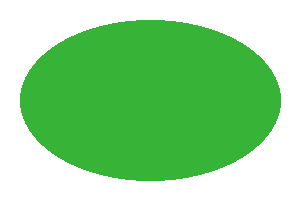
\includegraphics[width=.3\linewidth]{fig-alpha.png}}

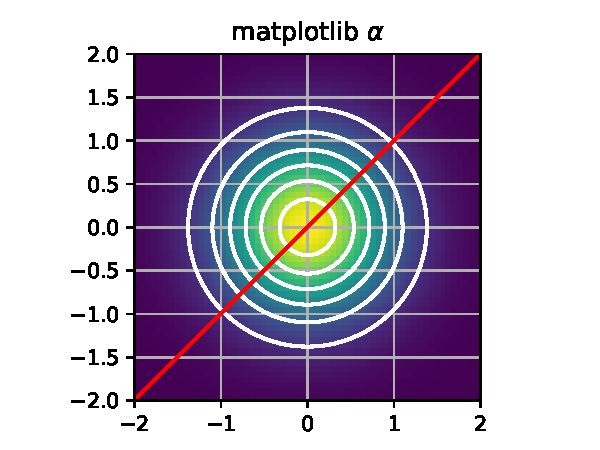
\includegraphics[width=.6\linewidth]{fig-mpl.pdf}


\includegraphics[width=.3\linewidth, trim=50 50 50 50, clip]{fig-a.png}
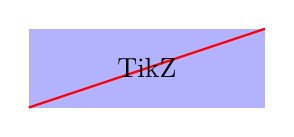
\begin{tikzpicture}\fill[blue!30] (0,0) rectangle (3,1); \draw[red, thick] (0,0) -- (3,1); \node at (1.5,.5) {TikZ};\end{tikzpicture}
\end{document}
